\thispagestyle{timhieukhoahocnone}
\pagestyle{timhieukhoahoc}
\everymath{\color{timhieukhoahoc}}
\blfootnote{$^1$\text{\color{timhieukhoahoc}Viện Sinh thái và Môi trường Đông Dương.}}
\graphicspath{{../timhieukhoahoc/pic2/}}
\begingroup
\AddToShipoutPicture*{\put(0,616){\includegraphics[width=19.3cm]{../bannertimhieu}}}
\AddToShipoutPicture*{\put(108,522){\includegraphics[scale=1]{../tieude.pdf}}}
\centering
\endgroup
\vspace*{185pt}

\begin{multicols}{2}
	Nhân dịp năm mới Nhâm Dần, chúng ta hãy cùng Pi tìm hiểu về bộ lông vằn của hổ dưới góc nhìn của toán học ứng dụng hiện đại.
	\vskip 0.1cm
	$\pmb{1.}$ \textbf{\color{timhieukhoahoc}Giới thiệu}
	\begin{figure}[H]
		\vspace*{-5pt}
		\centering
		\captionsetup{labelformat= empty, justification=centering}
		\includegraphics[width= 1\linewidth]{1}
		\caption{\small\textit{\color{timhieukhoahoc}Hình $1$. Bộ lông của loài hổ.}}
		\vspace*{-10pt}
	\end{figure}
	Hổ (tên khoa học \textit{Panthera tigris}) là loài động vật lớn nhất trong họ Mèo, phân bố ở nhiều khu vực châu Á như Sibera, Ấn Độ, Đông Nam Á và đảo Sumatra của Indonesia. Các nền văn hóa khác nhau đều có các sự tích giải thích về bộ lông vằn của chúng. Trong bài viết này, chúng ta hãy cùng tìm hiểu về mô hình toán học giải thích tại sao chúng lại có bộ lông độc đáo như vậy.
	\vskip 0.1cm
	$\pmb{2.}$ \textbf{\color{timhieukhoahoc}Mô hình phản ứng -- khuyếch tán}
	\vskip 0.1cm
	Alan Turing được nhiều người biết đến như một nhà khoa học tiên phong trong lĩnh vực khoa học máy tính, với những dấu ấn quan trọng trong sự phát triển của máy tính điện tử cũng như trí tuệ nhân tạo. Không chỉ vậy, năm $1951$, Turing chuyển sang nghiên cứu một lĩnh vực mới: toán học trong sinh học. Trong bài báo năm $1952$ (Turing, $1952$), ông đã đề xuất một mô hình toán học mà ông cho rằng có thể được sử dụng để giải thích cho các mẫu hoa văn xuất hiện trong tự nhiên.
	\begin{figure}[H]
		\vspace*{-5pt}
		\centering
		\captionsetup{labelformat= empty, justification=centering}
		\includegraphics[width= 0.65\linewidth]{2}
		\caption{\small\textit{\color{timhieukhoahoc}Alan Turing ($1912 - 1954$).}}
		\vspace*{-10pt}
	\end{figure}
	Mô hình của Turing có thể được giải thích một cách sơ lược như sau (Kondo \& Miura, $2010$):
	\vskip 0.1cm 
	$\bullet$ Giả sử trên một bề mặt (ví dụ da của động vật), có hai loại chất, được gọi là các morphogen (từ tiếng Latin: \textit{morpho} -- hình thái, \textit{gen} -- tạo ra). Đồng thời, trên bề mặt của ta xảy ra phản ứng tạo ra cả morphogen $1$ và morphogen $2$. 
	\vskip 0.05cm
	$\bullet$ Morphogen $1$ có tác dụng kích thích phản ứng, làm tăng nồng độ của nó lẫn morphogen $2$. Ta gọi morphogen $1$ là morphogen kích hoạt.
	\vskip 0.05cm
	$\bullet$ Morphogen $2$ có tác dụng ức chế phản ứng, làm giảm nồng độ của morphogen $1$ và chính nó. Ta gọi morphogen $2$ là morphogen ức chế.
	\vskip 0.05cm
	$\bullet$ Cả hai morphogen đều được khuyếch tán ra các vị trí xung quanh.
	Hai thành phần chính của mô hình trên bao gồm quá trình phản ứng và quá trình khuếch tán nên đây còn được gọi là mô hình phản ứng -- khuyếch tán.
	\vskip 0.05cm
	Với mỗi morphogen, Turing sử dụng một phương trình toán học để biểu diễn sự thay đổi nồng độ của nó theo thời gian (các phương trình này yêu cầu một số kiến thức toán cao cấp, các chi tiết liên quan có thể tham khảo trong phần phụ lục của (Kondo \& Miura, $2010$)). Các phân tích toán học trong bài báo của Turing cho thấy hệ phương trình trên có 6 trạng thái ổn định về nồng độ morphogen (Hình $2$): 
	\begin{figure}[H]
		\vspace*{-5pt}
		\centering
		\captionsetup{labelformat= empty, justification=centering}
		\includegraphics[width= 1\linewidth]{3}
		\caption{\small\textit{\color{timhieukhoahoc}Hình $2$. Các trường hợp của trạng thái ổn định của mô hình phản ứng -- khuyếch tán, biểu diễn cho miền mô phỏng một chiều.}}
		\vspace*{-10pt}
	\end{figure}
	I. Đồng đều trong toàn môi trường	
	\vskip 0.05cm
	II.	Dao động đồng pha giữa hai ngưỡng cố định
	\vskip 0.05cm
	III. Sóng dừng với bước sóng rất ngắn
	\vskip 0.05cm
	IV.	Dao động với bước sóng rất ngắn
	\vskip 0.05cm
	V. Dao động với bước sóng hữu hạn
	\vskip 0.05cm
	VI.	Sóng dừng với bước sóng hữu hạn
	\vskip 0.05cm
	Trong các trường hợp trên, trường hợp VI đáng chú ý nhất do nó có thể giải thích việc tạo thành các hoa văn cố định trên bề mặt. Ta có thể giải thích một cách định tính cho trường hợp này như sau (Hình $3$): 
	\begin{figure}[H]
		\vspace*{-5pt}
		\centering
		\captionsetup{labelformat= empty, justification=centering}
		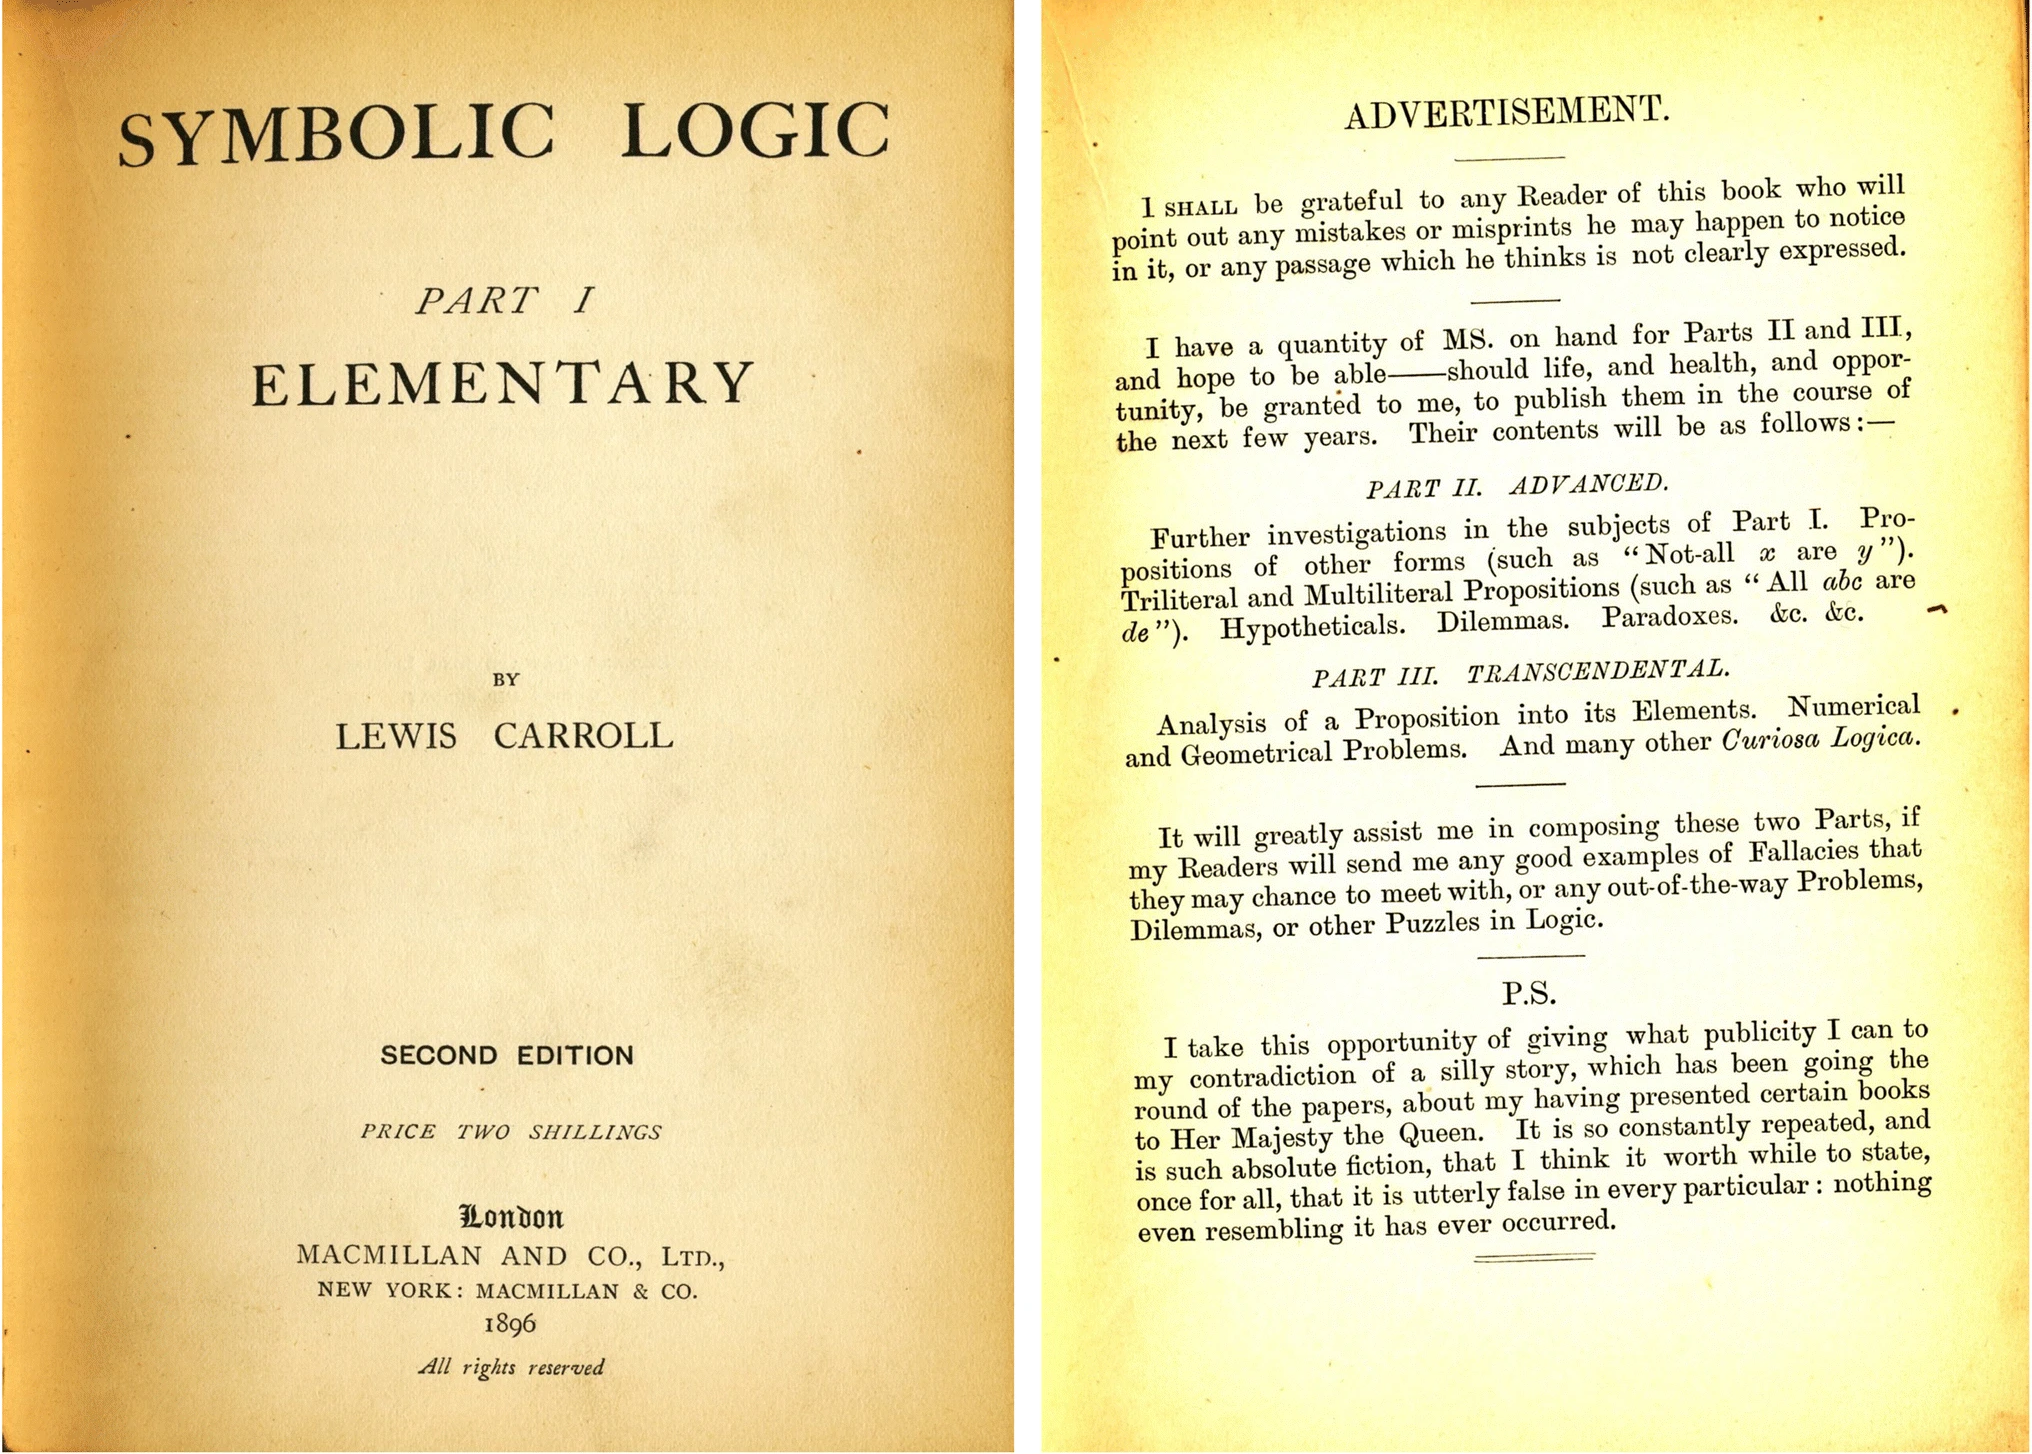
\includegraphics[width= 1\linewidth]{4}
		\caption{\small\textit{\color{timhieukhoahoc}Hình $3$. Minh họa cho trường hợp VI trong miền một chiều. Đường nét liền là nồng độ của morphogen kích hoạt. Đường nét đứt là nồng độ của morphogen ức chế.}}
		\vspace*{-10pt}
	\end{figure}
	$1.$ Tại một vị trí, morphogen kích hoạt có nồng độ cao hơn so với các vị trí xung quanh.
	\vskip 0.05cm
	$2.$ Tại vị trí nồng độ morphogen kích hoạt cao hơn thì phản ứng cũng xảy ra mạnh hơn (đây còn gọi là cơ chế tự tăng cường của morphogen kích hoạt). Do đó, cả morphogen tăng cường và morphogen ức chế cũng được sinh ra nhiều hơn.
	\vskip 0.05cm
	$3.$ Morphogen ức chế có khả năng khuếch tán mạnh hơn (đây là một đặc điểm quan trọng của trường hợp này) và do đó khi khuếch tán sẽ làm giảm mức độ phản ứng cũng như nồng độ morphogen kích hoạt tại các vị trí xung quanh (vùng A trong hình).
	\vskip 0.05cm
	$4.$ Nồng độ morphogen kích hoạt giảm tại các vùng A cũng làm giảm nồng độ morphogen ức chế sinh ra; đồng thời lượng morphogen ức chế được khuếch tán đến các vùng xa hơn (vùng B trong hình) cũng sẽ giảm.
	\vskip 0.05cm
	$5.$ Tại các vùng B, do nồng độ morphogen ức chế giảm, phản ứng sẽ xảy ra mạnh hơn làm tăng nồng độ morphogen kích hoạt ở đây. Sự tương tác giữa các vị trí theo cơ chế này có thể dẫn đến trạng thái dừng với dạng lồi lõm khác nhau của đồ thị.
	\vskip 0.05cm
	Sau khi sử dụng một số xấp xỉ tuyến tính để đơn giản hóa hệ phương trình, Turing đã giải bài toán cho một bộ số liệu cụ thể và thu được một kết quả với dạng vệt loang như trong Hình $4$. 
	\begin{figure}[H]
		\vspace*{-5pt}
		\centering
		\captionsetup{labelformat= empty, justification=centering}
		\includegraphics[width= 0.5\linewidth]{5}
		\caption{\small\textit{\color{timhieukhoahoc}Hình $4$. Kết quả tính toán của Turing. Đoạn thẳng nhỏ biểu diễn một đơn vị độ dài trong mô hình.}}
		\vspace*{-10pt}
	\end{figure}
	Ngày nay hệ phương trình phản ứng -- khuyếch tán của Turing có thể giải trực tiếp trên máy tính với các phương pháp số hiện đại. Kết quả thu được với các điều kiện và tham số khác nhau cho ta các mẫu hoa văn đa dạng như trong hình. Những mẫu dạng này còn được biết đến với tên gọi các mẫu Turing (Turing pattern). 
	\begin{figure}[H]
		\vspace*{-5pt}
		\centering
		\captionsetup{labelformat= empty, justification=centering}
		\includegraphics[width= 1\linewidth]{6}
		\caption{\small\textit{\color{timhieukhoahoc}Hình $5$. Một số mẫu Turing với các đường nét hoa văn đa dạng (Kondo $\&$ Miura, $2010$).}}
		\vspace*{-10pt}
	\end{figure}
	Cùng giai đoạn với nghiên cứu lý thuyết của Turing thì nhà hóa học Liên Xô, Boris Belousov, cũng phát hiện những dao động đều do quá trình phản ứng gây ra. Khi ông gửi đăng những kết quả này thì đều bị từ chối vì các phản biện cho rằng hiện tượng này là không thể xảy ra. Trong những năm $1960$, một nhà hóa học Nga khác là Anatol Zhabotinsky phát hiện rằng một phản ứng tương tự như của Belousov có thể cho ra các mẫu vạch sọc trong quá trình phản ứng xảy ra. Công bố này cũng không gây được ảnh hưởng gì lớn vào lúc đó.
	\vskip 0.05cm
	Cùng lúc đó trong ngành sinh học, mô hình của Turing cũng không được nhắc đến. Vào giai đoạn những năm $1960$, sinh học phát triển trở thành một chủ đề được quan tâm với nhiều nghiên cứu về việc các tế bào của phôi động vật hình thành các bộ phận cơ thể khác nhau như thế nào. Nhà sinh học Lewis Wolpert tiến hành các nghiên cứu trên phôi gà, một đối tượng dễ nhân giống và thuận tiện để quan sát. Ông đưa ra một mô hình chỉ có một morphogen: các tín hiệu được phát ra và lan truyền bằng khuếch tán từ một vị trí. Các tế bào sẽ tiến hành phát triển dựa trên nồng độ của chất này xung quanh mình. Wolpert lấy ví dụ về sự phát triển ngón ở cánh gà. Trong thực tế, gà có $3$ ngón rất nhỏ ở mỏm cánh. Theo giải thích của Wolpert, morphogen được phát ra từ một bên mép và khuếch tán. Tùy theo nồng độ của morphogen mà các ngón sẽ có hình thái khác nhau: ngón út, ngón giữa và ngón trỏ. Mô hình ``thông tin theo vị trí" này còn được gọi là thuyết gradient morphogen (Hình $6$). Thuyết này càng được tin tưởng khi thí nghiệm cấy ghép đảo chiều vùng tạo morphogen làm cho các ngón ở cánh gà cũng đảo chiều.
	\begin{figure}[H]
		\vspace*{-5pt}
		\centering
		\captionsetup{labelformat= empty, justification=centering}
		\includegraphics[width= 1\linewidth]{8}
		\caption{\small\textit{\color{timhieukhoahoc}Hình $6$. Mô hình của Wolpert về gradient morphogen ở cánh gà. $a)$ Vùng phát triển ngón. $b)$ Mô hình vùng tạo morphogen và vị trí tạo các ngón. $c)$ Hình ảnh ba ngón ở cánh gà. $d)$ Các ngưỡng morphogen khác nhau cho hình thái khác nhau. Wolpert ví sự tách biệt này giống như lá cờ~Pháp.}}
		\vspace*{-10pt}
	\end{figure}
	Phải đến năm $1979$, hai nhà khoa học là Stuart Newman và Harry Frisch mới đưa ra một cách giải thích khác sử dụng mô hình Turing (Newman \& Frisch, $1979$). Theo đó, việc hình thành các ngón xảy ra theo cơ chế tạo thành mẫu Turing (các ngón tương ứng với các sọc trong mẫu) còn cơ chế gradient morphogen xảy ra sau đó sẽ định hình các đặc tính (độ dài ngắn, ...) của ngón. 
	\vskip 0.05cm
	Ý tưởng của Newman ban đầu được nhiều người chú ý đến. Tuy nhiên, thuyết Wolpert đã giữ một vị trí thống trị trong sinh học phát triển của phôi một thời gian tương đối dài. Mô hình toán học với các phương trình phản ứng -- khuyếch tán cũng có vẻ quá phức tạp với các nhà sinh học. Những người ủng hộ Wolpert cũng gây áp lực lớn để ngăn chặn mô hình mới được cho là ngược với những gì họ tin tưởng. Các nghiên cứu sau đó của Newman không được các tạp chí chấp nhận. Ông cũng không còn được mời tham gia các hội thảo khoa học. Khi một nghiên cứu khác cho thấy các vạch quan sát được ở phôi của ruồi giấm là kết quả của tổ hợp các gen kích hoạt tạo nên gradient morphogen giống với mô hình Wolpert, nghiên cứu của Newman cũng như mô hình Turing có vẻ như không còn cơ hội trong ngành sinh học phát triển.
	\begin{figure}[H]
		\vspace*{-5pt}
		\centering
		\captionsetup{labelformat= empty, justification=centering}
		\includegraphics[height= 0.48\linewidth]{9a}\quad
		\includegraphics[height= 0.48\linewidth]{9b}
		\caption{\small\textit{\color{timhieukhoahoc}Hình $7$. Trái: các vạch sọc dạng mẫu Turing (trường hợp VI ở phần trước) trong phản ứng Belousov -- Zhabontinsky (Bourgine $\&$ Annick Lesne, $2011$). Phải: các sóng tròn đồng tâm (trường hợp V) trong phản ứng Belousov -- Zhabotinsky (Ball, $2015$).}}
		\vspace*{-10pt}
	\end{figure}
	Phải đến một thập kỷ sau, vào năm $1990$, công trình nghiên cứu của một nhóm nhà hóa học Pháp lại cung cấp các bằng chứng về mô hình Turing trong các phản ứng hóa học tương tự phản ứng Belousov -- Zhabotinsky. Sự kiện này cũng đánh dấu cho sự trở lại của thuyết phản ứng -- khuếch tán trong sinh học.
	\vskip 0.05cm
	$\pmb{3.}$ \textbf{\color{timhieukhoahoc}Các bằng chứng mới từ sinh học phát triển và di truyền}
	\vskip 0.05cm
	Trong số các loài cá có hoa văn, giống cá \textit{Pocamanthus}, thuộc họ Cá bướm gai, có một đặc điểm đặc biệt: các hoa văn trên người chúng thay đổi dần theo độ tuổi với sự khác biệt rõ rệt ở các giai đoạn.
	\begin{figure}[H]
		\vspace*{-5pt}
		\centering
		\captionsetup{labelformat= empty, justification=centering}
		\includegraphics[height= 0.20\linewidth]{10a}
		\includegraphics[height= 0.202\linewidth]{10b}
		\includegraphics[height= 0.20\linewidth]{10c}\\
		
		\vspace*{2pt}
		\includegraphics[height= 0.2\linewidth]{10d}
		\includegraphics[height= 0.2\linewidth]{10e}
		\includegraphics[height= 0.2\linewidth]{10f}
		\caption{\small\textit{\color{timhieukhoahoc}Hình $8$. Trên: Ba giai đoạn từ nhỏ đến trưởng thành của loài Pocamanthus imperator; từ vằn tròn chuyển dần thành sọc. Dưới: Ba giai đoạn tương ứng của Pocamanthus semicirculatus; từ vạch chuyển sang vòng rồi cuối cùng là đốm.}}
		\vspace*{-10pt}
	\end{figure}
	Nghiên cứu của Shigeru Kondo năm $1995$ trên \textit{Pocamanthus imperator} (Kondo \& Asai, $1995$) cho thấy ở các vị trí được mô phỏng, quá trình biến đổi của vân trên cơ thể cá cũng giống với kết quả diễn biến theo thời gian của nồng độ morphogen khi mô phỏng bằng hệ phương trình phản ứng -- khuếch tán (Hình~$9$).
	\begin{figure}[H]
		\vspace*{-5pt}
		\centering
		\captionsetup{labelformat= empty, justification=centering}
		\includegraphics[width= 1\linewidth]{11}
		\caption{\small\textit{\color{timhieukhoahoc}Hình $9.$ So sánh đường vân của cá nuôi với kết quả mô phỏng. Nửa trên: vị trí gần mang cá. Nửa dưới: vị trí gần đuôi.}}
		\vspace*{-10pt}
	\end{figure}
	Những nghiên cứu tiếp theo của Kondo tiến hành trên cá ngựa vằn, một sinh vật được sử dụng phổ biến ở các phòng thí nghiệm sinh học cho thấy khi dùng laser tẩy một phần sọc vằn của cá, quá trình phục hồi trên da cá giống với kết quả mô phỏng (Kondo, Watanabe, \& Miyazawa, $2021$) (Hình $10$).
		\begin{figure}[H]
		\vspace*{-5pt}
		\centering
		\captionsetup{labelformat= empty, justification=centering}
		\includegraphics[width= 1\linewidth]{12}
		\caption{\small\textit{\color{timhieukhoahoc}Hình $10$. Trên: Da cá ngựa vằn bị tẩy một phần sọc và quá trình phục hồi sọc. Dưới: kết quả mô~phỏng.}}
		\vspace*{-10pt}
	\end{figure}
	Một điểm đáng chú ý là sự hình thành sọc vằn ở cá ngựa vằn xảy ra không phải do phản ứng -- khuếch tán giữa các morphogen mà là do tương tác giữa hai loại tế bào trên da cá. Tuy cơ chế sinh học là khác nhưng ta vẫn có thể sử dụng hệ phương trình như mô hình của Turing để biểu diễn nó!
	\begin{figure}[H]
		\vspace*{-10pt}
		\centering
		\captionsetup{labelformat= empty, justification=centering}
		\includegraphics[height= 0.4\linewidth]{13a}
		\includegraphics[height= 0.4\linewidth]{13b}
		\caption{\small\textit{\color{timhieukhoahoc}Hình $11$. Thí nghiệm khi tắt một số gen ở phôi chuột làm tăng số lượng ngón chân. Trái: bàn chân chuột trong thí nghiệm. Phải: Kết quả mô~phỏng.}}
		\vspace*{-10pt}
	\end{figure}
	Vấn đề về liên hệ giữa quá trình phát triển chi và ngón với mô hình Turing cũng được nghiên cứu trở lại. Ở chuột, thí nghiệm khi một số gen liên quan đến quá trình phát triển ngón bị tắt đi, số lượng ngón chân của phôi chuột lại tăng lên (Sheth et al., $2012$) (Hình $11$). Hiện tượng này không  thể giải thích được theo mô hình Wolpert nhưng lại phù hợp với kết quả mô phỏng dùng mô hình Turing. Các ngón chân trong trường hợp này cũng xòe ra và nhỏ hơn, tạo hình quạt giống với vây cá. Kết quả nghiên cứu này cho thấy khi vây của cá tiến hóa thành bàn chân ở các loài sau này, sự thay đổi của các gen làm thay đổi tham số của hệ phương trình phản ứng -- khuếch tán. Toán học thật là kì diệu, với cùng một hệ phương trình, ta được nghiệm là vây cá với một bộ tham số và nghiệm là bàn chân chuột với một bộ tham số khác!
	\begin{figure}[H]
		\vspace*{-5pt}
		\centering
		\captionsetup{labelformat= empty, justification=centering}
		\includegraphics[width= 1\linewidth]{14a}
		\includegraphics[width= 1\linewidth]{14b}
		\includegraphics[width= 1\linewidth]{14c}
		\caption{\small\textit{\color{timhieukhoahoc}Hình $12.$ Trên: Mô hình BSW về phát triển bàn chân ở phôi chuột. Mũi tên nét liền đầu nhọn thể hiện quan hệ tăng cường. Mũi tên nét liền đầu bằng thể hiện quan hệ ức chế. Mũi tên nét đứt thể hiện quan hệ điều tiết thông qua tham số. $k_1$, $...$, $k_9$ là các tham số của hệ phương trình gắn với quá trình tương tác tương ứng. Giữa: Kết quả mô phỏng sự phát triển bàn chân ở phôi chuột. Dưới: Kết quả thí nghiệm quan sát được về sự phát triển bàn chân ở phôi chuột.}}
		\vspace*{-10pt}
	\end{figure}
	Trong nghiên cứu tiếp theo, bằng cách thử các tổ hợp gen mã hóa các protein khác nhau, người ta đã xác định được các protein khác liên quan đến quá trình tạo thành bàn chân ở chuột (Raspopovic, Marcon, Russo, \& Sharpe, $2014$). Theo đó có $3$ protein đóng vai trò morphogen (thay vì $2$ như trong mô hình đã trình bày) đồng thời có hai protein khác (Hoxd$13$ và Fgf) đóng vai trò điều tiết tham số của mô hình tại các vị trí trong không gian. Sự tham gia của các protein điều tiết này giống với mô hình của Wolpert. Khi đó hệ phương trình của ta sẽ có ba phương trình thay vì $2$. Kết quả mô phỏng dựa trên mô hình này cũng khớp với quá trình phát triển bàn chân ở phôi chuột.
	\vskip 0.05cm
	Mô hình Turing còn được kiểm chứng qua các hiện tượng liên quan đến lai tạo. Ở cá bảy màu, một loài cá cảnh phổ biến, phần đuôi của chúng thường có nhiều loại hoa văn khác nhau do quá trình lai và chọn giống. Nhiều mẫu hoa văn trong số này có thể mô phỏng lại được bằng hệ phương trình phản ứng -- khuyếch tán.
	\begin{figure}[H]
		\vspace*{-6pt}
		\centering
		\captionsetup{labelformat= empty, justification=centering}
		\includegraphics[width= 1\linewidth]{15}
		\caption{\small\textit{\color{timhieukhoahoc}Hình $13$. Các mẫu Turing và hoa văn ở cá bảy~màu.}}
		\vspace*{-12pt}
	\end{figure}
	Nghiên cứu di truyền trên cá nóc cũng cho thấy các loài có hoa văn dạng mê cung là kết quả của sự lai ghép giữa các loài có đốm trắng (trên nền có màu) và loài có đốm màu (trên nền trắng). Trong mô hình thì tham số của các loài lai này cũng ứng với những giá trị trung gian của các loài đốm trên (Miyazawa, $2020$). Điều này cũng thể hiện đặc điểm phi tuyến tính của mô hình phản ứng -- khuếch tán.
	\vskip 0.05cm
	Các nghiên cứu trên cùng nhiều nghiên cứu khác đã giúp đưa mô hình Turing trở lại với ngành sinh học. Đặc biệt, trong giai đoạn hiện nay, sự kết hợp giữa nghiên cứu hình thái học, di truyền học và toán học (nhất là mô phỏng) là cần thiết để giải đáp những vấn đề phức tạp về sự phát triển của sinh vật.
	\begin{figure}[H]
		\vspace*{5pt}
		\centering
		\captionsetup{labelformat= empty, justification=centering}
		\includegraphics[width= 0.9\linewidth]{16}
		\caption{\small\textit{\color{timhieukhoahoc}Hình $14$. Mô hình Turing và di truyền ở cá nóc.}}
		\vspace*{-10pt}
	\end{figure}
	$\pmb{4.}$ \textbf{\color{timhieukhoahoc}Mẫu Turing ở các sinh vật họ Mèo}
	\vskip 0.05cm
	Ta hãy trở lại với câu chuyện về vằn ở hổ. Trong họ Mèo, trừ những loài màu trơn như sư tử, ta có thể quan sát thấy các mẫu Turing ở hổ và một số loài khác với những cấu trúc đa dạng: sọc vằn, đốm, khoang, ... 
%	\vskip 0.05cm
	\begin{figure}[H]
		\vspace*{-5pt}
		\centering
		\captionsetup{labelformat= empty, justification=centering}
		\includegraphics[width=1\linewidth]{h15}
		\caption{\small\textit{\color{timhieukhoahoc}Hình $15$. Mẫu Turing ở một số loài họ Mèo. Từ trên xuống: hổ, báo cheetah, báo hoa (leopard).}}
		\vspace*{-3pt}
	\end{figure}
	\begin{figure}[H]
		\vspace*{5pt}
		\centering
		\captionsetup{labelformat= empty, justification=centering}
		$a)$\includegraphics[width= 0.95\linewidth]{18}
		$b)$\includegraphics[height= 0.29\linewidth]{18b}
		$c)$\includegraphics[height= 0.29\linewidth]{18c}
		\caption{\small\textit{\color{timhieukhoahoc}Hình $16$. $a)$ Mô phỏng của Murray về mẫu Turing ở phần đuôi một số loài họ Mèo. $b)$ Genetta genetta.  $c)$ Đột biến ở báo cheetah.}}
		\vspace*{-10pt}
	\end{figure}
	Về cơ bản, loài họ Mèo nào có hoa văn thì đều có một lượng vằn nhất định, ít nhất là ở đuôi. Theo các mô phỏng của Murray (Murray, $2002$), kích thước phôi lúc các mẫu Turing được hình thành (tương ứng với miền mô phỏng cho hệ phương trình) sẽ quyết định loại hình dạng nào của hoa văn chiếm ưu thế. Với các loài có kích thước nhỏ, ví dụ \textit{Genetta genetta}, toàn bộ đuôi là sọc vằn trong khi cơ thể là đốm. Với các loài kích thước lớn hơn như báo cheetah hay báo đốm (jaguar) thì các họa tiết \,hoa/đốm chiếm phần lớn đuôi. Ở báo hoa thì số lượng sọc vằn ở chóp đuôi rất ít. Cũng theo Murray, việc hổ chỉ có vằn mà không có đốm dù kích thước cơ thể lớn có thể là do quá trình hình thành các vân xảy ra ở thời điểm sớm trong quá trình phát triển phôi. Một trường hợp được giải thích tương tự là một dạng đột biến của báo cheetah với các sọc dài ở lưng, chuyển dần thành đốm ở chân. Theo đó, đột biến sẽ đẩy sớm thời gian bắt đầu xuất hiện của các mẫu Turing. Khi đó phôi còn nhỏ nên chỉ có sọc vằn xuất hiện từ các vị trí dọc theo lưng và chuyển dần sang đốm ở các vị trí khác khi phôi tăng trưởng. Với mèo nhà, do không bị áp lực cạnh tranh sinh tồn nên các giai đoạn phát triển của phôi cũng không bị cố định chặt chẽ như các loài họ mèo trong tự nhiên. Do vậy, bộ lông của mèo nhà đa dạng hơn nhiều với nhiều kiểu hoa văn và màu sắc khác nhau.
	\vskip 0.2cm
	\PIbox{\textbf{\color{timhieukhoahoc}Màu lông của hổ}
		\vskip 0.05cm
		Một vấn đề cũng khiến nhiều người băn khoăn là tại sau lông hổ lại có màu da cam trong khi chúng sống ở trong rừng rậm với môi trường màu xanh lá cây. Trong thực tế, hổ và các loài mà nó săn bắt đều có các tế bào thị giác chỉ nhìn được hai màu (thay vì ba màu như ở người). Với chúng thì  phổ màu từ màu xanh lá cây đến đỏ đều trông giống nhau. Đồng thời, ở các loài thú, màu da cam dễ tổng hợp hơn màu xanh lá cây mà vẫn đảm bảo được việc ngụy trang.}
	\vskip 0.2cm
	$\pmb{5.}$ \textbf{\color{timhieukhoahoc}Một số mẫu Turing khác trong tự nhiên}
	\vskip 0.05cm
	Ở các loài thú, mẫu Turing có thể có những dạng đơn giản như nửa đên nửa trắng, khoang màu, cho đến các loại sọc và loang phức tạp hơn.
	\begin{figure}[H]
		\vspace*{-5pt}
		\centering
		\captionsetup{labelformat= empty, justification=centering}
		$a)$\includegraphics[height= 0.32\linewidth]{19a}
		$b)$\includegraphics[height= 0.32\linewidth]{19b}
		$c)$\includegraphics[height= 0.32\linewidth]{19c}
		$d)$\includegraphics[height= 0.32\linewidth]{19d}
		$e)$\includegraphics[height= 0.32\linewidth]{19e}
		$f)$\includegraphics[height= 0.32\linewidth]{19f}
		\caption{\small\textit{\color{timhieukhoahoc}Hình $17.$ Mẫu Turing ở một số loài thú. $a)$ Lửng. $b)$ Dê Valais. $c)$ Thú ăn kiến. $d)$ Bò khoang. $e)$ Ngựa vằn $f)$ Hươu cao cổ.}}
		\vspace*{-10pt}
	\end{figure}  
	Bên cạnh các loài cá đã nhắc đến ở phần $3$, ta cũng có thể quan sát thấy mẫu Turing ở nhiều loài cá khác. Ở thực vật, một số nghiên cứu cũng cho thấy mẫu Turing có liên quan đến các hoa văn trên lá cây, hoa, ... 
	\vskip 0.05cm
	Các mẫu Turing còn xuất hiện trên các bộ phận cơ thể của động vật: vỏ ốc, cánh bướm, lông chim, phân bố của râu chuột, vảy bò sát, ... Ở cơ thể người, quá trình lành các vết thương, sự hình thành các phân nhánh trong phổi,  cũng được một số nghiên cứu mô phỏng dùng mô hình phản ứng -- khuếch tán.
	\begin{figure}[H]
		\vspace*{-5pt}
		\centering
		\captionsetup{labelformat= empty, justification=centering}
		$a)$\includegraphics[height= 0.34\linewidth]{21a}
		$b)$\includegraphics[height= 0.34\linewidth]{21b}
		$c)$\includegraphics[height= 0.34\linewidth]{21c}
		$d)$\includegraphics[height= 0.34\linewidth]{21d}
		$e)$\includegraphics[width=0.91\linewidth]{21e}
		\caption{\small\textit{\color{timhieukhoahoc}Hình $20$. Mẫu Turing xuất hiện ở các bộ phận cơ thể động vật. $a)$ vỏ ốc $b)$ cánh bướm $c)$ lông chim $d)$ phân bố của râu chuột $e)$ vảy bò sát.}}
		\vspace*{-10pt}
	\end{figure}  
	$\pmb{7.}$ \textbf{\color{timhieukhoahoc}Lời kết}
	\vskip 0.05cm
	Mô hình khuếch tán -- phản ứng là một trong những ứng dụng quan trọng của toán học trong sinh học. Đồng thời, nó cũng cho thấy vẻ đẹp của toán học trong sự gắn kết với tự nhiên và đời sống. Sự kết hợp của toán học và các ngành khoa học khác sẽ góp phần giải mã nhiều bí ẩn khác trong tương lai. Các mẫu Turing cũng là một chủ đề hấp dẫn khi chọn hướng nghiên cứu cho các độc giả chuyên ngành Toán.
	\vskip 0.05cm
	\textbf{\color{timhieukhoahoc}Tài liệu tham khảo}
	\vskip 0.05cm
	[$1$] Kondo, S., \& Asai, R. ($1995$). A reaction--diffusion wave on the skin of the marine angelfish Pomacanthus. \textit{Nature}, $376(6543)$, $765-768$.
		 \url{https://doi.org/10.1038/376765a0}
	\vskip 0.05cm
	[$2$] Kondo, S., \& Miura, T. ($2010$). Reaction--Diffusion Model as a Framework for Understanding Biological Pattern Formation. \textit{Science}, $329(5999)$, $1616-1620$. \url{https://doi.org/10.1126/science.117} \url{9047}
	\vskip 0.05cm
	[$3$] Kondo, S., Watanabe, M., \& Miyazawa, S. ($2021$). Studies of Turing pattern formation in zebrafish skin. \textit{Philosophical Transactions of the Royal Society A: Mathematical, Physical and Engineering Sciences}, $379(2213)$.
		 \url{https://doi.org/10.1098/rsta.2020.0274}
	\vskip 0.05cm
	[$4$] Miyazawa, S. ($2020$). Pattern blending enriches the diversity of animal colorations. \textit{Science Advances}, $6(49)$.
		 \url{https://doi.org/10.1126/sciadv.abb9107}
	\vskip 0.05cm
	[$5$] Murray, J. D. ($2002$). Mathematical biology. New York: Springer.
	Newman, S. A., \& Frisch, H. L. ($1979$). Dynamics of Skeletal Pattern Formation in Developing Chick Limb. \textit{Science}, $205(4407)$, $662-668$.
		 \url{https://doi.org/10.1126/science.462174}
	\vskip 0.05cm
	[$6$]Raspopovic, J., Marcon, L., Russo, L., \& Sharpe, J. ($2014$). Digit patterning is controlled by a Bmp-Sox$9$-Wnt Turing network modulated by morphogen gradients. \textit{Science}, $345(6196)$, $566-570$.
		 \url{https://doi.org/10.1126/science.1252960}
	\vskip 0.05cm
	[$7$] Sheth, R., Marcon, L., Bastida, M. F., Junco, M., Quintana, L., Dahn, R., ... Ros, M. A. ($2012$). Hox Genes Regulate Digit Patterning by Controlling the Wavelength of a Turing--Type Mechanism. \textit{Science}, $338(6113)$, $1476-1480$. 
		\url{https://doi.org/10.1126/science.1226804}
	\vskip 0.05cm
	[$8$] Turing, A. ($1952$). The chemical basis of morphogenesis. \textit{Philosophical Transactions of the Royal Society of London. Series B, Biological Sciences}, $237(641)$, $37-72$.
		 \url{https://doi.org/10.1098/rstb.1952.0012}
\end{multicols}